\documentclass[11pt]{article}
\usepackage[T1]{fontenc}
\usepackage[utf8]{inputenc}
\usepackage{multirow}
\usepackage{graphicx}
\graphicspath{ {images/} }
\usepackage[table,xcdraw]{xcolor}
\usepackage{listings}
\usepackage{hyperref}
\usepackage{pgfgantt}
\usepackage{vmargin}
\usepackage{wrapfig}
\usepackage{enumitem}
\usepackage{subfiles}
\usepackage{multirow}
\usepackage{float}
\usepackage{url}

\setlength\parindent{0pt}

\setpapersize{A4}
\setmargins{2.5cm}  % margen izquierdo
{1.5cm}             % margen superior
{16.5cm}            % anchura del texto
{23.42cm}           % altura del texto
{10pt}              % altura de los encabezados
{1cm}               % espacio entre el texto y los encabezados
{0pt}               % altura del pie de p�gina
{2cm}               % espaci\title{Determinitzaci� d'un aut�mat finit}


\definecolor{barblue}{RGB}{153,204,254}
\definecolor{groupblue}{RGB}{51,102,254}
\definecolor{linkred}{RGB}{165,0,33} 

\author{José Miguel Avellana López}
\date{6 de Julio del 2021}

\def\contentsname{Index}
\begin{document}
	
	\setcounter{tocdepth}{4}
	\setcounter{secnumdepth}{4}
	
	\begin{titlepage}
		\begin{figure}[htb]
			\begin{center}
				
\includegraphics[width=7cm]{logoUDL.png}
				\vspace*{\stretch{1.0}}
				\\
				\medskip
				\begin{center}
					\noindent\rule{16.5cm}{0.4pt}
					\linebreak 
					\\
					\Huge\textbf {Sistema distribuido para la resolución de problemas SAT}
					\noindent\rule{16.5cm}{0.4pt}
					\hfill\\
					\Large\textbf\textit{Informe de Seguimiento}
					%\noindent\rule{16.5cm}{0.4pt}
					\\
					\bigskip
					\hfill\\
					\hfill\\
					\hfill\\
					\hfill\\
					\hfill\\
					\hfill\\
					\hfill\\
					\setlength{\parskip}{1em}
				\end{center}
				\vspace*{\stretch{2.0}}
			\end{center}
		\end{figure}
		\begin{flushright}
			Universitat de Lleida
			\\
			Escola Politécnica Superior
			\\
			Grau en Enginyeria Informática
			\\
			\medskip
			\hfill\\
			\normalsize\textbf{Autor:}
			\\
			\large\textit{Jose Miguel Avellana López}
			\\
			\normalsize\textbf{Codirector:}
			\\
			\large{Josep Luis Lérida Monsó}
			\\
			\normalsize\textbf{Codirector:}
			\\
			\large{Josep Argelich Romá}
		\end{flushright}
		\thispagestyle{empty} 
	\end{titlepage}
	\thispagestyle{empty}
	\newpage
		\renewcommand*\listfigurename{Index de figures}
		\thispagestyle{empty}
		\renewcommand*\listtablename{Index de taules}
		\thispagestyle{empty}
	\newpage
	
	\section{Evolución del trabajo}
		Los puntos principales en los que se dividió el proyecto durante el informe inicial fueron:
		\begin{itemize}
			\item Definir, de manera simple, 
				las reglas básicas de cada uno de los componentes de un sistema distribuido de servicios,
				y como se definen e interaccionan entre sí.
			\item Dar uso del sistema para realizar una prueba concepto sobre un problema concreto, la resolución de problemas SAT. \leavevmode \\
		\end{itemize}
		De esto, el primer punto, la especificación de las reglas básicas del sistema, se puede dar por terminado puesto que,
		aunque es posible que se requiera alguna modificación durante el período restante,
		se ha desarrollado hasta el punto de permitir la ejecución del segundo punto. \\ 

		El segundo punto, el desarrollo de una solución a un problema concreto (resolución de SAT), ha sido desarrollado parcialmente.
		Esto cubre dos desarrollos paralelos, por un lado el aplicativo del nodo y por otro los servicios para clasificar
		y resolver solvers. \\

		Por la parte del nodo, actualmente es posible construir y ejecutar servicios. A su vez, se ha implementado la lógica requerida para registrar
		todos los servicios levantados por el nodo, creando un árbol de dependencias para poder detener aquellos cuyo padre haya sido detenido, tanto para 
		servicios solicitados localmente como por pares (otros nodos).
		Queda, por tanto, implementar la lógica para que los nodos sean capaces de:
		\begin{itemize}
			\item Encontrar e identificar otros nodos de la red.
			\item Balancear la construcción de nuevas instancias de servicios. \\
		\end{itemize}

		Por la parte del servicio de clasificación, se han completado los tres puntos acordados en el informe inicial, estos eran:
		\begin{itemize}
			\item Cargar especificaciones de SAT-solvers, pedirle al nodo que le devuelva
			 instancias de los mismos y mantenerlos (comprobar que siguen activos).
			\item Clasificar los SAT-solvers que se le han especificado.
			\item Seleccionar un SAT-solver en función de un cnf dado.
		\end{itemize}
		Conviene la realización de varios puntos más, a saber:
		\begin{itemize}
			\item Balanceo de carga de las solicitudes sobre la resolución de cnf's.
			\item Comprobar, dando uso de solvers modificados para realizar la prueba, el correcto funcionamiento tanto de la clasificación como de la regresión del modelo. \leavevmode \\
		\end{itemize}

		Sobre el balanceo de instancias y peticiones en el clasificador, se debe de tener en cuenta que:
		\begin{itemize}
			\item Por un lado, el clasificador debe de levantar tantas instancias de un solver como se necesite entre el nodo local y sus pares.
				(El balanceo de instancias es
				responsabilidad del nodo, él decide en que nodo de la red se ejecuta cada instancia).
			\item Por otro lado, el balanceo de peticiones para resolver cnf's corre a cargo del servicio de clasificación, ya que es a éste al que lo solicita 
				el cliente.
				El servicio de clasificación, por tanto, deberá seleccionar el solver más óptimo para el cnf dado y, tras esto, seleccionar la instancia de dicho
				solver con menos carga en ese momento.
		\end{itemize}

		Además de lo mencionado anteriormente, también hay que tener en cuenta la necesidad de
		realizar múltiples solicitudes al servicio de clasificación. Sobre esto cabe preguntarse:
	
		¿Cómo realizan múltiples clientes solicitudes al servicio de clasificación? \\

		En base a la arquitectura anteriormente desarrollada, si un cliente quiere dar uso de un servicio, éste solicita la creación de una instancia del mismo a su nodo,
		por lo tanto, si n clientes quieren dar uso del servicio, serán necesarias n instancias de éste, a fin de cuentas, la instancia de un servicio, un contenedor, no es
		más que un hilo aislado. 
		Por lo tanto, el paradigma cliente/servidor se ve alterado al hablar de servicios distribuidos. En vez de un servidor atendiendo múltiples clientes, un cliente solicita
		el despliegue de un servicio. 
		En términos de rendimiento no debería existir una gran diferencia entre un esquema y otro, puesto que el servidor centralizado termina ejecutando n hilos para n solicitudes
		de clientes, en los servicios distribuidos estos hilos se aislan (esto puede ser un punto negativo sobre el uso de memoria compartida) 
		y se reparten entre los nodos de la red. \\

		Ahora bien, en caso de querer realizar un servicio web, al que poder, tal vez, conectar con un frontend en un navegador, será necesario un nuevo servicio el cual se encargue
		de recibir las solicitudes de los clientes y desplegar y dar uso del servicio de clasificación. 
		Este servicio por tanto, puede ser comprendido como un puente entre la "web tradicional" y una red de servicios distribuidos.
		
		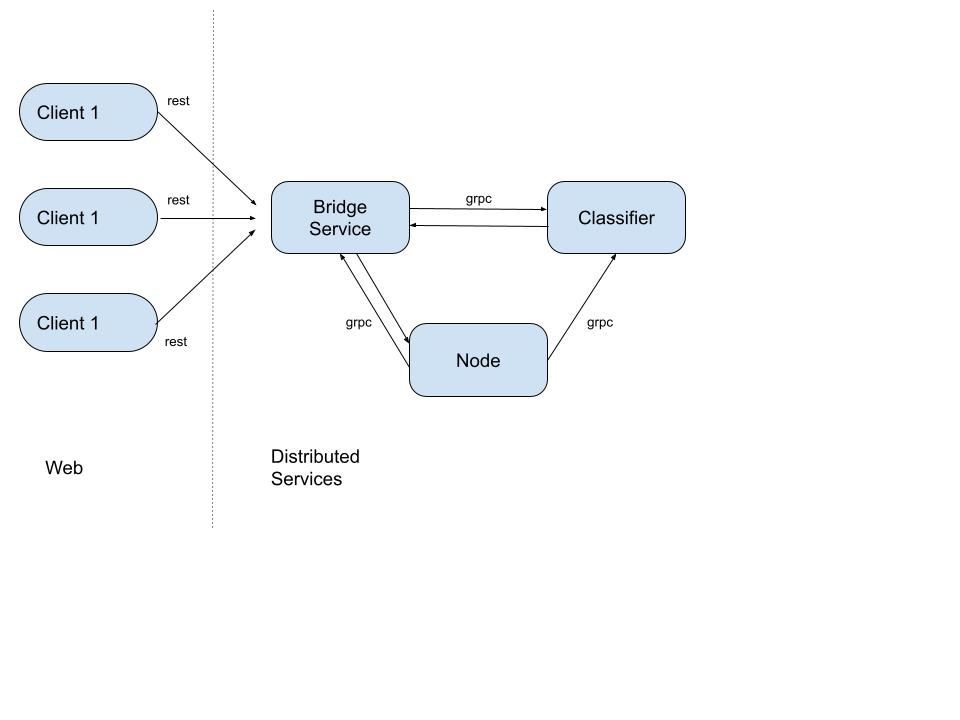
\includegraphics[width=16cm]{Esquema_puente.jpg}

	\section{Decisiones técnicas que se han tomado}
		\subsection{Varias instancias no pueden compartir dependencias}
			La naturaleza que adopta la red crea una jerarquía de instancias de servicios repartidas entre los nodos de la mísma. \\
			Esto significa que, cuando una instancia (padre) solicita una instancia de otro servicio (hijo), este último
			pasará a ser dependiente del primero, adoptando el padre el derecho a decidir cuando debe de morir el hijo y la responsabilidad
			sobre su consumo de recursos (en caso en que un nodo realice un seguimiento del consumo de cada instancia, deberá tener en cuenta el de sus dependencias).
			De esta forma, si se mata al padre, el nodo donde se este ejecutando su hijo podrá matarlo. \\
			Si no fuera asi, un nodo no sabría que instancias quedan en estado 'zombie' ya que ninguno de sus clientes 
			(instancias padre) se haría responsable.

		\subsection{Comunicación nodo-servicio}
			Definir como debe comportarse un sistema requiere abordar cuales son los deberes y derechos de sus componentes. \\

			Un nodo debe de proporcionar una interfaz con la que los servicios puedan comunicarse, junto con la dirección
			a la que el servicio le realizará sus solicitudes. La forma en la que el nodo carga estos componentes en una nueva instancia
			es mediante un archivo binario en la raiz del sistema de ficheros del servicio. Esto es así ya que el servicio podría requerir de
			estos datos antes de levantar su servidor. \\

			Ante la solicitud de una nueva instancia, un nodo tiene el derecho de, o bien construir esta instancia localmente, o bien solicitarle la instancia
			a un par (otro nodo). Así mismo, el nodo tiene el deber de retornar tanto una dirección con la que comunicarse con la nueva instancia, como un token
			para realizar acciones sobre ella al solicitante.
			En caso de crear la dependencia de un servicio en un par, el nodo debe de asegurarse que el solicitante tenga acceso a la dirección que le otorga para
			comunicarse con su dependencia. \\

			Esta arquitectura permite a un servicio no preocuparse del nodo donde se ejecutará cada dependencia. Del mismo modo que los nodos no se preocuparán de
			la utilidad que puedan tener las instancias que ejecutan. \\
			
			Por tanto, para resumir, durante la construcción de la instancia de un servicio, el nodo añade en su raiz un binario que contiene como comunicarse con él.
			Si el servicio quiere dar uso de una dependencia, le enviará la especificación de ésta al nodo, y éste le devolverá una dirección con la que comunicarse y
			un token para poder matarla. Será el nodo el que busque donde construir esa dependencia, si localmente o en alguno de sus pares. También será el nodo el que,
			en caso de matar a la primera instancia, acabe con la segunda.

		\subsection{Serialización y topología de la especificación de un servicio}
			La especificación de un servico se serializa en un binario Protobuf. \\

			Está compuesto por los siguientes elementos:
			\begin{itemize}
				\item hash: Lista de hashes (del tipo sha256:913ref3...) sobre el binario del resto de la especificación.
				\item Syntax: Sintaxis de la especificación.
				\item Container: Especifica el contenedor donde se ejecuta el servicio, esto es:
					\begin{itemize}
						\item la arquitectura, define el hardware y el kernel donde se debe de ejecutar el servicio.
						\item el punto de entrada, define la ruta del primer ejecutable del servicio.
						\item el sistema de archivos, representado en un árbol donde las hojas son los archivos en binario.
						\item las variables de entorno, lista compuesta por llave y definición del campo de cada variable. 
					\end{itemize} 
				\item Api: Define cómo se puede interactuar con el servicio, constituida por:
					\begin{itemize}
						\item interfaz de la aplicación (mensajes, métodos y errores y respuestas de cada uno).
						\item lista de slots, cada uno compuesto por los siguentes elementos:
							\begin{itemize}
								\item puerto donde escucha.
								\item protocolo de comunicación que soporta (HTTP/2, GRPC ...).
							\end{itemize}
					\end{itemize} 
				\item Tensor: Opcional. Definie la topología del modelo que entrena el servicio. Un servicio podría solicitar al nodo que le retorne las instancias
					de aquellos servicios que tengan un tensor determinado y con ellas realizar solicitudes a servicios que ya tienen el modelo entrenado.
			\end{itemize}
		\subsection{Json vs GRPC} 
			Json se ha convertido en prácticamente un estandar a la hora de compartir información en la web, debido a que es el sistema de serialización de Javascript, y éste, a su vez,
			es el lenguaje estandarizado para ejecutarse en los navegadores web. \\

			Pero en una red de microservicios, donde los entornos de ejecución son virtualizados, Javascript pierde protagonismo y, por tanto, Json también.
			Es por esto que cabe preguntarse cual es la mejor forma de serializar las comunicaciones entre servicios. Al ser evidente que no existe un protocolo capaz de
			liderar ni en cualquier ámbito ni indefinidamente, cada Slot de un servicio definirá el protocolo soportado. \\

			Concretamente para este proyecto se dará uso de Grpc, principalmente por dos razones:
			\begin{itemize}
				\item Protobuf, su lenguaje de serialización, consigue comprimir bytes de manera muy eficiente enfocando los buffers a cada topología de mensajes.
				\item Utiliza Http/2, por lo que está preparado para realizar streaming bidireccional de manera eficiente.
			\end{itemize}
			Otros protocolos tambien a tener en cuenta podrían ser Flatbuffers o Capt'n proto.

	\section{Evaluación crítica del estado del trabajo}
		En base a la planificación temporal del informe inicial, podemos concluir que existe cierto retraso en cuanto a la tercera 
		fase de desarrollo, la cual cubre todo lo mencionado anteriormente (balanceo de instancias, balanceo de solicitudes y conexión de nodos).

		Por lo tanto, con el fin de dejar margen a la redacción de la memoria, sería necesario terminar el desarrollo del trabajo en el mes de Julio. \\
		\\Reajuste del esquema de Gantt:

		\begin{ganttchart}[
			canvas/.append style={fill=none, draw=black!5, line width=.75pt},
			hgrid style/.style={draw=black!5, line width=0.75pt},
			vgrid={*1{draw=black!5, line width=.75pt}},
			today=18,
			today rule/.style={
				draw=black!64,
				dash pattern=on 3.5pt off 4.5pt,
				line width=1pt
			},
			today label font=\tiny,
			title/.style={
				draw=none, 
				fill=none
			},
			title label font=\tiny,
			title label node/.append style={below=7pt},
			include title in canvas=false,
			bar label font=\mdseries\small\color{black!70},
			bar/.append style={
				draw=none, 
				fill=barblue
			},
			bar progress label font=\mdseries\footnotesize\color{black!70},
		]{1}{18}
			\gantttitle{Noviem.}{2}
			\gantttitle{Diciem.}{2}
			\gantttitle{Enero}{2}
			\gantttitle{Febrero}{2}
			\gantttitle{Marzo}{2}
			\gantttitle{Abril}{2}
			\gantttitle{Mayo}{2}
			\gantttitle{Junio}{2}
			\gantttitle{Julio}{2}
			\gantttitle{Agosto}{2}\\
			\ganttbar[]{\textbf{Estudio previo}}{1}{2} \\
			\ganttbar[]{\textbf{Analisis de requisitos}}{3}{3} \\
			\ganttbar[]{\textbf{Primera fase de desarrollo}}{4}{6} \\
			\ganttbar[]{\textbf{Segunda fase de desarrollo}}{7}{11} \\
			\ganttbar[]{\textbf{Reunion inicial}}{10}{10} \\
			\ganttbar[]{\textbf{Tercera fase de desarrollo}}{15}{18} \\
			\ganttbar[]{\textbf{Reunion de Seguimiento}}{15}{15} \\
			\ganttbar[]{\textbf{Testing del sistema}}{7}{19} \\
			\ganttbar[]{\textbf{Redacción de la memoria}}{18}{20} \\
			\ganttbar[]{\textbf{Reunion final}}{20}{20} \\

		\end{ganttchart}

\end{document}



